% !TeX root = main.tex
\changecolours{ScoutGreen}
\section[Diagnóstico, Covered Queries e Benchmark]{Diagnóstico com \texttt{explain()}, \textit{Covered Queries} e Benchmark}

% ------------------------------------------------------------------------------
\begin{frame}[fragile]{Auditoria de Execução: Os Modos do \texttt{explain()}}
  \vspace{0.05cm}
  \begin{columns}[t]
    \begin{column}{0.48\textwidth}
      \alert{Níveis de Auditoria do Otimizador}\par
      \itemseps[topsepi=0.2mm,itemsepi=0.5mm,labelsep=1.5mm,leftmargini=2.5mm]
      \scriptsize
      \begin{itemize}
        \item \textbf{\texttt{queryPlanner} (Padrão):} Retorna apenas o plano eleito pelo otimizador sem executar a consulta.
        \item \textbf{\texttt{executionStats} (Recomendado):} Executa a consulta e retorna métricas reais de tempo, nós examinados e documentos lidos.
        \item \textbf{\texttt{allPlansExecution}:} Executa e documenta o desempenho de todos os planos candidatos testados.
      \end{itemize}
    \end{column}
    \begin{column}{0.48\textwidth}
      \alert{Sintaxe no MongoSH / PyMongo}\par
      \begin{lstlisting}[language=mongosh]
// Executando auditoria completa:
db.produtos.find(
  { sku: "SKU-INF-000101" }
).explain("executionStats")
      \end{lstlisting}
      \itemseps[topsepi=0.2mm,itemsepi=0.5mm,labelsep=1.5mm,leftmargini=2.5mm]
      \scriptsize
      \begin{itemize}
        \item Permite aos engenheiros de dados inspecionar se a consulta está usando índice (\texttt{IXSCAN}) ou colapsando em \texttt{COLLSCAN}.
      \end{itemize}
    \end{column}
  \end{columns}
\end{frame}

% ------------------------------------------------------------------------------
\begin{frame}{Decodificando as Quatro Métricas Vitais do \texttt{executionStats}}
  \vspace{0.05cm}
  \makebox[\textwidth][c]{%
    \scriptsize
    \renewcommand{\arraystretch}{1.22}
    \begin{tabular}{p{2.8cm} p{3.2cm} p{6.0cm}}
      \toprule
      \textbf{Métrica no JSON} & \textbf{Conceito Técnico} & \textbf{Alvo de Otimização} \\
      \midrule
      \texttt{stage} & Estágio da árvore de execução. & \texttt{IXSCAN} (Sem \texttt{COLLSCAN} ou \texttt{SORT} em RAM). \\
      \texttt{totalDocsExamined} & Documentos físicos lidos do disco/cache. & Deve aproximar-se de \texttt{nReturned} (ou 0). \\
      \texttt{totalKeysExamined} & Nós da $B\text{-Tree}$ inspecionados. & Próximo a \texttt{nReturned} (afunilamento eficiente). \\
      \texttt{nReturned} & Documentos realmente devolvidos. & Volume útil solicitado pela aplicação. \\
      \texttt{executionTimeMillis} & Tempo de processamento em ms. & $\le 1\text{ ms}$ para operações pontuais. \\
      \bottomrule
    \end{tabular}%
  }
  \vspace{0.15cm}
  \centering{\scriptsize \textbf{Razão de Eficiência:} $\displaystyle \frac{\text{totalDocsExamined}}{\text{nReturned}} \quad (\text{Ideal} = 1.0; \quad \text{COLLSCAN sob } 50.000 \text{ itens} = 5.000)$.}
\end{frame}

% ------------------------------------------------------------------------------
\begin{frame}[fragile]{\textit{Covered Queries} (Consultas Cobertas): O Santo Graal da Performance}
  \vspace{0.05cm}
  \begin{columns}[t]
    \begin{column}{0.48\textwidth}
      \alert{O que é uma Consulta Coberta?}\par
      \itemseps[topsepi=0.2mm,itemsepi=0.5mm,labelsep=1.5mm,leftmargini=2.5mm]
      \scriptsize
      \begin{itemize}
        \item Todos os campos da consulta (filtro e projeção) estão presentes no próprio índice $B\text{-Tree}$.
        \item O MongoDB \textbf{NUNCA lê o documento BSON do disco}!
        \item O estágio \textbf{\texttt{FETCH}} desaparece, operando 100\% em memória RAM com \textbf{\texttt{totalDocsExamined: 0}}!
      \end{itemize}
    \end{column}
    \begin{column}{0.48\textwidth}
      \alert{Código da Consulta Coberta}\par
      \scriptsize
      \begin{lstlisting}[language=mongosh]
// 1. Criar indice cobrindo categoria, preco e sku:
db.produtos.createIndex({
  categoria: 1,
  preco: 1,
  sku: 1
})

// 2. Consulta 100% coberta:
// ATENCAO: _id: 0 eh OBRIGATORIO para evitar o FETCH!
db.produtos.find(
  { categoria: "Informática", preco: { $lte: 1500 } },
  { categoria: 1, preco: 1, sku: 1, _id: 0 }
).explain("executionStats")
      \end{lstlisting}
    \end{column}
  \end{columns}
\end{frame}

% ------------------------------------------------------------------------------
\begin{frame}{Resultados do Benchmark no Laboratório (50.000 Documentos)}
  \vspace{-0.1cm}
  \begin{figure}[htbp]
    \centering
    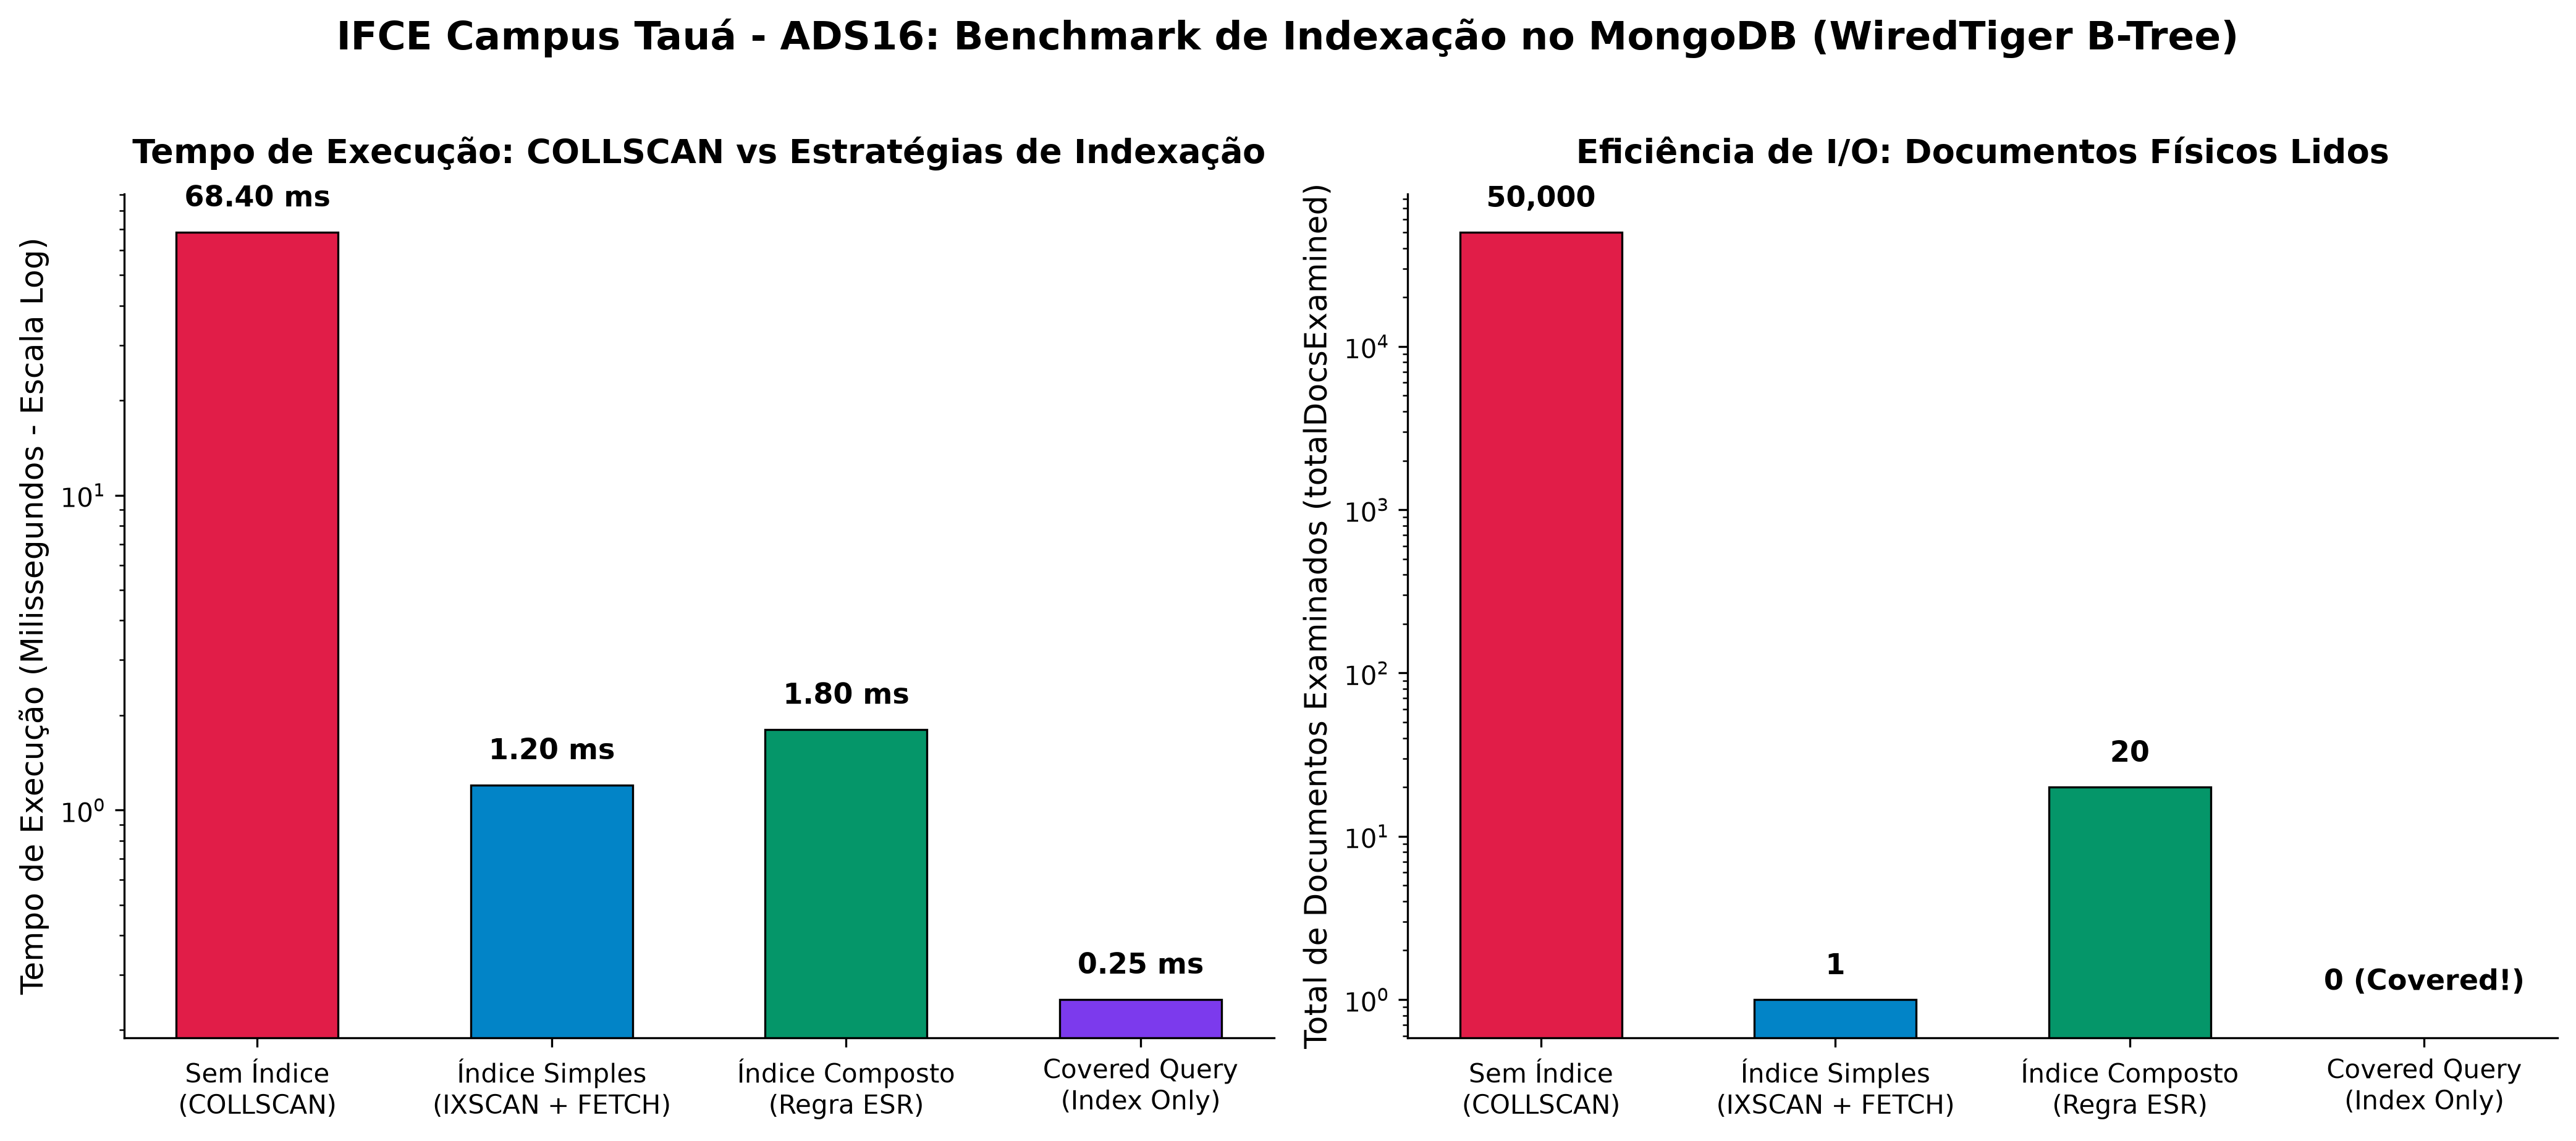
\includegraphics[width=0.90\textwidth,height=0.68\textheight,keepaspectratio]{benchmark_performance_indices.png}
  \end{figure}
  \vspace{-0.3cm}
  \centering{\tiny \textbf{Conclusão:} Adoção de índices compostos (ESR) e consultas cobertas reduz a latência em mais de $99.7\%$ e zera leituras físicas de documentos.}
\end{frame}
